\documentclass[11pt,a4paper]{article}

\usepackage[UTF8]{ctex}
\usepackage[margin=2.35cm]{geometry}
\usepackage{amsmath,amssymb,amsfonts}
\usepackage{booktabs}
\usepackage{multirow}
\usepackage{array}
\usepackage{graphicx}
\usepackage{subcaption}
\usepackage{algorithm}
\usepackage{algorithmic}
\usepackage[numbers,sort&compress]{natbib}
\usepackage{xcolor}
\usepackage{enumitem}
\usepackage{hyperref}
\usepackage{url}
\usepackage{xurl}

\hypersetup{
    colorlinks=true,
    linkcolor=blue!65!black,
    citecolor=blue!65!black,
    urlcolor=blue!65!black
}

\setlist[itemize]{leftmargin=1.8em}
\setlist[enumerate]{leftmargin=1.8em}
\renewcommand{\arraystretch}{1.12}
\newcolumntype{P}[1]{>{\raggedright\arraybackslash}p{#1}}
\urlstyle{tt}

\newcommand{\method}{SkyCausal}
\newcommand{\cmax}{C_{\max}}
\newcommand{\E}{\mathbb{E}}
\newcommand{\Var}{\operatorname{Var}}
\newcommand{\confirmed}{\textcolor{green!45!black}{\textbf{[已确认]}}}
\newcommand{\development}{\textcolor{orange!80!black}{\textbf{[开发证据]}}}
\newcommand{\pending}{\textcolor{red!70!black}{\textbf{[待确认]}}}
\newcommand{\todo}[1]{\textcolor{red!70!black}{\textbf{[TODO: #1]}}}

\title{
    \textbf{\method：面向连续物理时钟动态 FJSP--MAPF 的\\
    开放式、截止期安全求解器组合元调度}\\[0.4em]
    \large
    \textit{Open and Deadline-Safe Solver-Portfolio Meta-Scheduling\\
    for Dynamic FJSP--MAPF under a Continuous Physical Clock}
}

\author{吴昊 \and \todo{补充合作者与单位}}
\date{内部迭代稿 v0.3（2026-08-11，30 状态在线开发版）}

\begin{document}
\maketitle

\begin{center}
\fcolorbox{orange!70!black}{orange!8}{
\parbox{0.92\linewidth}{
\textbf{证据说明。}
本文是随实现与实验共同演化的论文首稿。
\confirmed 表示已有冻结独立确认支持；
\development 表示仅用于方法筛选的开发实验；
\pending 表示方法或结论尚未通过独立确认。
开发结果不得替代论文主实验。
}}
\end{center}

\begin{abstract}
柔性作业车间调度（FJSP）决定工序的机器与加工顺序，多智能体路径规划（MAPF）
决定自动导引车能否按时、无碰撞地完成工件运输。两者在动态制造环境中形成闭环：
调度计划产生时空运输需求，而拥堵、绕行、机器故障和实际到达时间又会改变后续
可行调度。现有方法通常固定一个求解器、在封闭的联合算法集合中做一次选择，或在
求解期间冻结物理状态，难以同时处理候选开放性、严格计算预算和计划新鲜度。

本文研究连续物理时钟下的在线求解器组合元调度问题，并提出 \method{} 框架。
系统以版本化 manifest、参数 schema、能力声明和统一 adapter 构成开放 Solver
Catalog；将 solver、配置、预算和切换能力统一表示为动态 SolverOption；使用短探测
收集首次可行解、目标值、下界、改进速度和停滞等灰盒信息，再以浅层 Root MCTS 或
逐轮淘汰分配探测预算。与展开未来制造状态的深层搜索不同，Root MCTS 只决定下一段
计算预算交给哪个候选。求解期间工厂继续运行；提交前，系统在最新物理状态上执行
freshness 检查、时间重对齐、独立可行性审计和原子激活，任何失败均保留当前安全计划。
此外，本文将 ``保持当前计划''、solver 和 probe budget 统一为候选动作，并以
状态条件执行价值 \(Q(s,o)\) 预测候选对剩余完整 episode 的影响，而非仅比较
FJSP makespan。

\confirmed 在冻结的六个联合 profile、40 个独立状态和既定 deadline policy 下，
早期 \(T=1\) Root Search 相对全局最佳固定 profile 将 held-out capped terminal
makespan 平均降低 23.575（4.88\%），95\% 分层 bootstrap 置信区间为
\([8.625,46.325]\)，且全部 deadline、清理和物理安全门槛通过。
\development 在随后 50 个连续时钟在线开发 episode 中，三个 FJSP solver 在不同
状态进入最优集合；匹配短预算下，makespan-only 选择的平均 regret 为 40.0，
透明 ridge 执行价值诊断为 9.2。然而该诊断只有 5 个独立状态，当前仅允许 shadow
运行，不能作为最终质量结论。
\development 在统一 keep-current/solver/config/budget 动作 schema 后，30 个独立
状态、7 种策略的 210 个配对在线 episode 表明：原始 MCTS 相对 keep-current
平均减少 5.5 步，但置信区间跨 0；为 CP-SAT 增加最小可辨识预算后，首轮可行覆盖由
0/30 提升为 28/30、最终选择 CP-SAT 15 次，但平均终局反而比原始 MCTS 差 7.8 步。
这表明恢复候选覆盖仍不足以优化在线终局。
\pending 后续独立确认将检验开放候选、freshness 过滤、执行价值和 Root MCTS 的
组合是否稳定优于固定 solver 与逐轮淘汰。
\end{abstract}

\noindent\textbf{关键词：}
柔性作业车间调度；多智能体路径规划；求解器组合；在线算法选择；MCTS；
灰盒赛马；滚动重调度

\section{引言}
\label{sec:introduction}

\subsection{研究背景}

在柔性制造系统中，一个工件通常需要依次访问多台机器。FJSP 负责决定工序在哪台
兼容机器上加工及其先后顺序；当相邻工序位于不同机器时，AGV 或移动机器人必须在
共享路网中运输工件。调度与运输因此不是可以独立优化的两个后处理阶段：

\begin{equation}
\begin{aligned}
    \text{机器与时序决策}
    &\rightarrow
    \text{运输任务释放}
    \rightarrow
    \text{无碰撞路径执行}\\
    &\rightarrow
    \text{实际到达与拥堵反馈}
    \rightarrow
    \text{后续机器和工序状态}.
\end{aligned}
\end{equation}

若 FJSP 只使用静态距离矩阵，则可能产生三类耦合损失：一是忽略真实运输成本的
距离盲区；二是计划到达时间与实际路径执行不一致的时序错位；三是运输任务在狭窄
区域集中释放导致的拥堵聚集。已有 FJSP-运输资源和冲突规避研究逐步提高了联合建模
强度~\citep{berterottiere2024fjsptransport,sun2023integrated}，但动态制造系统还
面临另一个问题：没有单一 FJSP 或 MAPF 求解器在所有状态、预算和拓扑下占优。

MAPF 算法选择研究已经显示，候选算法及其超参数会随实例而改变优劣
~\citep{ren2021mapfast,alkazzi2022mapfaster,chen2024nopanacea,
shabalin2024mag}。动态 FJSP 研究也开始从固定规则转向状态依赖的启发式组合
~\citep{chen2025dyromcts,huang2026dsevolve}。然而，将这类选择机制用于闭环
FJSP--MAPF 仍存在三个未被同时解决的问题。

\subsection{核心挑战}

\paragraph{开放候选。}
固定六个或若干人工枚举的 FJSP--MAPF profile 适合复现实验，却不适合作为长期
动作空间。新增 solver、超参数或预算不应要求修改控制器固定输出维度。

\paragraph{连续物理时钟。}
如果影子求解时冻结工厂，求得的方案可能在真实提交时已经过期。在线元搜索必须在
机器加工、AGV 移动和维修计时持续推进时运行，并把探测、切换、清理和提交开销全部
计入端到端墙钟预算。

\paragraph{执行价值。}
较小的残余 FJSP makespan 不等价于较好的在线终局。机器分配会改变运输距离、任务
集中度和拥堵结构；长时间 probe 也可能因状态漂移而抵消更优的离线目标值。因此，
最终选择应评价候选在当前状态下的完整执行价值，而不是只看 solver 的内部目标。

\subsection{研究问题}

本文关注如下问题：

\begin{quote}
在动态 FJSP--MAPF 制造系统中，当当前安全计划继续执行且物理时钟持续推进时，
能否在严格端到端预算内，从可扩展的 solver/config/budget 候选中分配短探测预算，
识别仍可安全提交且具有较高执行价值的方案，并在失败时无副作用地保留当前计划？
\end{quote}

\subsection{贡献与证据边界}

本文的贡献按当前证据状态表述如下。

\begin{enumerate}
    \item \textbf{连续时钟在线元调度问题与协议。}
    本文将候选求解、物理执行和计划提交放入同一时间语义，明确区分事件状态、
    提交状态、求解器预算和 commit reserve，并给出 failure-as-cost、原子激活和
    安全 fallback 规则。\confirmed 六 profile \(T=1\) 基线已完成独立确认。

    \item \textbf{开放 Solver Catalog 与动态 SolverOption。}
    候选由 solver identity、版本、配置、预算、资源和能力组成；新增 solver 通过
    manifest、schema、adapter 和 calibration 接入，不修改控制器固定类别数。
    \development 当前已接入 CP-SAT、DE 和 PSO 的真实 FJSP probe；开放 MAPF
    meta selection 仍为 \pending。

    \item \textbf{用于探测预算分配的浅层 Root MCTS。}
    MCTS 不展开未来制造状态树，而是在根节点上把下一段 probe 预算分配给候选，
    结合渐进扩展、灰盒进度、失败成本和 deadline fallback。
    \pending 其相对逐轮淘汰的正式收益尚未确认。

    \item \textbf{提交安全与状态条件执行价值。}
    本文提出 ``可行性过滤 \(\rightarrow\) 最新状态 freshness/rebase
    \(\rightarrow\) 执行价值排序'' 的决策顺序，并将 keep-current 纳入动作空间。
    \development 初步结果否定了 makespan-only；执行价值模型当前只以 shadow
    方式采集和评估。
\end{enumerate}

\section{相关工作}
\label{sec:related}

\subsection{FJSP、运输资源与动态联合调度}

FJSP with Transportation Resources 显式考虑加工与运输资源共享
~\citep{berterottiere2024fjsptransport}。Sun 等将柔性车间调度与无冲突路径结合
~\citep{sun2023integrated}。Li 等研究含 AGV 的实时柔性车间调度，并采用多智能体
强化学习联合任务、机器和车辆决策~\citep{li2025realtime}。这些工作说明生产物流
必须联合考虑，但其动作通常是制造资源决策，而本文动作是 solver/config/budget
及其生命周期管理；两类方法互补，不能在缺少同协议基线时直接声称全面优越。

DyRo-MCTS 将 MCTS 用于动态作业车间的 job-selection，并以离线策略作为 prior
~\citep{chen2025dyromcts}。本文不把 ``使用 MCTS'' 视为创新：其差异在于只进行
根节点 probe 预算分配，并显式处理 FJSP--MAPF solver、连续物理时钟、远程请求
清理和提交新鲜度。

\subsection{MAPF 算法选择与组合}

MAPFAST 和 MAPFASTER 学习从 MAPF solver portfolio 中选择较快算法
~\citep{ren2021mapfast,alkazzi2022mapfaster}。No Panacea 将选择扩展到次优 solver、
不同超参数以及 runtime-quality 权衡~\citep{chen2024nopanacea}；MAG 使用图嵌入
表示 MAPF 实例~\citep{shabalin2024mag}。这些方法主要在求解前做一次选择，而本文
还使用求解过程中的灰盒进度，并要求候选计划在持续变化的制造状态上重新验证。

LNS2+RL 在一次 MAPF 求解中前期使用较高质量的学习型 replanner、后期切换到更快的
优先级规划器~\citep{wang2025lns2rl}，说明 continue/switch 不应被限制为算法外部的
一次性动作。本文通过统一 start、observe、stop、export 和 cleanup 契约，为 solver
原生混合或控制器编排预留接口。

\subsection{灰盒配置与 anytime portfolio}

实时灰盒算法配置利用 solver 中间输出提前停止不具潜力的配置
~\citep{weiss2025graybox}。Anytime portfolio 进一步表明，单一配置难以覆盖不同
运行时预算，solver、配置与预算应共同构成候选~\citep{schede2026anytime}。
本文吸收上述思想，但优化目标不是独立 benchmark 上的 solver runtime 或内部目标，
而是候选在闭环制造 episode 中的执行成本。

\subsection{动态启发式组合}

DSevolve 离线构造行为多样的动态 FJSP 规则档案，并利用 probe fingerprint 在线
检索~\citep{huang2026dsevolve}。本文同样强调多样候选与短 probe，但候选可以是
异构精确、启发式和 MAPF solver；执行层还必须处理绝对 deadline、跨服务清理、
portable incumbent 与最新物理状态兼容性。DSevolve 当前为预印本，本文仅将其作为
趋势证据。

\section{问题定义}
\label{sec:problem}

\subsection{闭环 FJSP--MAPF 系统}

设作业集合为 \(\mathcal{J}\)，机器集合为 \(\mathcal{M}\)，AGV 集合为
\(\mathcal{A}\)，车间路网为 \(G=(V,E)\)。作业 \(J_i\) 包含有序工序
\(O_{i1},\ldots,O_{in_i}\)。工序 \(O_{ij}\) 可在机器集合
\(\mathcal{M}_{ij}\subseteq\mathcal{M}\) 上加工，在机器 \(m\) 上的加工时间为
\(p_{ijm}\)。机器一次最多加工一个工序，已开始加工的工序不可撤销。

当相邻工序被分配到不同位置时，系统释放 pickup-delivery 运输任务。AGV 路径是
顶点和时间的序列，联合路径不得发生顶点冲突或反向边冲突。实际到达时间决定后继
工序是否可开始，因此终局 makespan 为
\begin{equation}
    \cmax = \max_{J_i\in\mathcal{J}} C_i,
\end{equation}
其中 \(C_i\) 包含加工、等待、运输、拥堵和恢复开销。

\subsection{动态事件与不可撤销前缀}

本文首先研究机器故障事件。事件 \(e_t\) 在物理时间 \(t\) 触发后，状态被划分为：
\begin{itemize}
    \item 已完成工序；
    \item 已开始加工、不可抢占的工序；
    \item 已装载运输和进入安全关键区的路径段；
    \item 尚未开始、允许重新规划的残余工序集合 \(\mathcal{R}_t\)。
\end{itemize}

实验状态捕获必须 action-independent：是否进入 cohort 只能由事件类型、物理可行性
和安全范围决定，不能依据某个 solver 的表现筛选。

\subsection{状态、候选与灰盒进度}

事件状态写作
\begin{equation}
    s_t =
    \left(
    X_t^{\mathrm{job}},
    X_t^{\mathrm{machine}},
    X_t^{\mathrm{agv}},
    X_t^{\mathrm{task}},
    G,
    e_t,
    \mathcal{R}_t
    \right).
\end{equation}

一个可执行候选不是单纯的算法名称，而是
\begin{equation}
    o =
    \left(
    d,\,
    id,\,
    v,\,
    \theta,\,
    b,\,
    r,\,
    \kappa
    \right),
    \label{eq:solveroption}
\end{equation}
其中 \(d\) 是 FJSP 或 MAPF 域，\(id,v\) 是 solver identity 与版本，
\(\theta\) 是参数，\(b\) 是探测预算，\(r\) 是资源需求，\(\kappa\) 是
start/observe/continue/switch/export 等能力。特殊候选 \(o^{\mathrm{keep}}\)
表示不提交新计划。

候选在第 \(k\) 次 probe 后产生灰盒进度
\begin{equation}
    z_{o,k} =
    \left(
    t_{\mathrm{first}},\,
    f_k,\,
    \ell_k,\,
    g_k,\,
    v_k,\,
    h_k,\,
    \xi_k
    \right),
\end{equation}
分别表示首次可行解时间、当前目标、下界、gap、改进速度、停滞时间和失败信号。

\subsection{连续时钟与预算约束}

元搜索开始后，物理工厂继续执行当前安全计划。设端到端预算为 \(B\)，选择阶段预算
为 \(B_{\mathrm{search}}\)，提交保留为 \(B_{\mathrm{commit}}\)，则
\begin{equation}
    B_{\mathrm{search}} + B_{\mathrm{commit}} \le B.
\end{equation}
探测、停止、导出、认证、清理、重对齐和激活都计入 \(B\)。未在截止期前完成的
候选不会部分激活，其失败以预注册成本计入。

\subsection{优化目标}

对当前状态与候选，定义剩余 episode 执行价值
\begin{equation}
    Q(s_t,o,z_o,\mathcal{B}_o)
    =
    \E\!\left[
        C_{\mathrm{remain}}
        \mid s_t,o,z_o,\mathcal{B}_o
    \right],
    \label{eq:qvalue}
\end{equation}
其中 \(\mathcal{B}_o\) 是认证 incumbent bundle。若预测均值和不确定性分别为
\(\mu_o,\sigma_o\)，风险成本可写为
\begin{equation}
    \widehat{c}_o = \mu_o + \beta\sigma_o.
\end{equation}

控制器目标是在严格预算和安全约束下最小化终局制造成本、选择 regret 与失败风险。
确定性的可行性和 freshness 检查优先于学习评分；模型不得授权本来不可提交的计划。

\section{\method{} 方法}
\label{sec:method}

\subsection{总体架构}

\begin{figure*}[t]
\centering
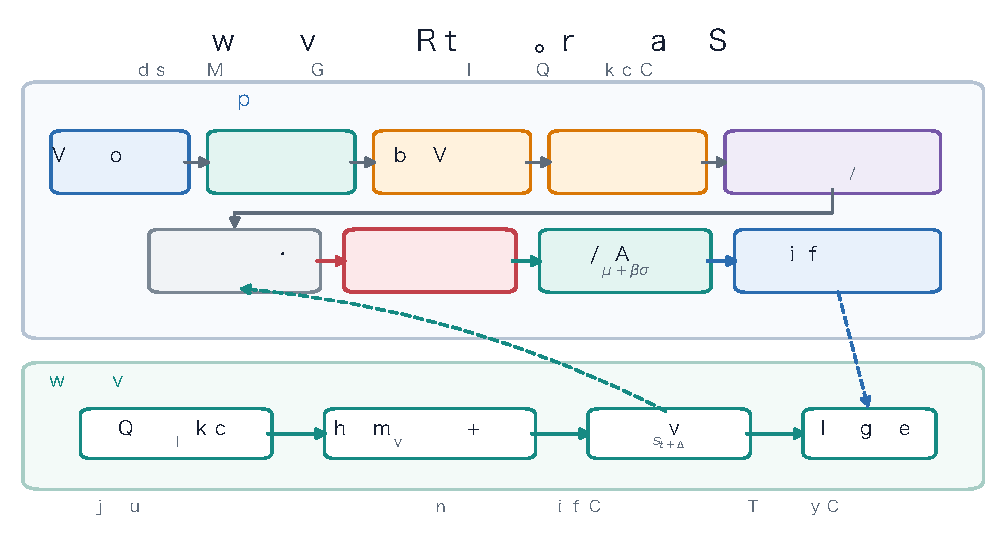
\includegraphics[width=\textwidth]{figures/v3/fig01_system_architecture.pdf}
\caption{\method{} 总体架构。上层由开放 Solver Catalog 生成
solver/config/budget 候选，以短 probe 采集灰盒轨迹，并由 Root MCTS 或逐轮淘汰分配
后续探测预算；下层制造系统在整个搜索期间持续执行当前认证计划。提交前先读取最新
物理状态并确定性删除未通过 freshness/rebase 的 bundle，再由 shadow \(Q\) 排序，
最后原子激活或执行 keep-current。}
\label{fig:overview}
\end{figure*}

图~\ref{fig:overview} 将元搜索与物理执行分成两个并行泳道。Root MCTS 的输出不是
最终计划，而是 probe 预算分配；候选只有在最新物理状态上通过 freshness/rebase 后
才进入价值排序和激活阶段。该边界避免把学习评分误写成安全认证。

\subsection{开放 Solver Catalog}

每个 solver 通过版本化 manifest 注册，至少声明：
\begin{equation}
\begin{split}
    \mathcal{D}_{\mathrm{solver}} = \{&
    id,\; version,\; domain,\; image\ digest,\; protocol,\\
    &config\ schema,\; capabilities,\; safe\ boundaries,\; resources
    \}.
\end{split}
\end{equation}
Catalog 按 domain、capability、资源和事件兼容性过滤候选。配置合法性由 solver 自身
schema 校验，控制器不维护求解器专用参数白名单。新增 solver 依次经过
contract、shadow、portfolio 和 transfer 四级准入。

\subsection{分解式候选生成}

若 FJSP 与 MAPF 候选数分别为 \(n_F,n_M\)，直接展开全部配置和预算的笛卡尔积会造成
组合爆炸。本文采用分解式生成：
\begin{equation}
    \mathcal{O}_t =
    \operatorname{ComposeTopK}
    \left(
        \operatorname{TopK}_F(s_t),
        \operatorname{TopK}_M(s_t,\pi_F)
    \right).
\end{equation}
FJSP 候选先产生带运输需求的 schedule proposal，MAPF 候选再按地图、AGV、任务波和
质量要求条件生成。\development 当前在线主流程已完成 FJSP 动态候选；
\pending MAPF 的开放 meta selection 尚未进入主实验。

\subsection{短探测与灰盒信息}

统一 adapter 提供
\begin{equation}
    \{\texttt{start},\texttt{observe},\texttt{stop},
      \texttt{export},\texttt{cleanup}\}.
\end{equation}
每次 probe 使用绝对 deadline，并预留 cooperative finalization 时间。只有通过独立
schedule audit 的 bundle 才可进入候选集。基础设施错误与算法无解分开记录，但二者
都不能产生部分提交。

\subsection{浅层 Root MCTS}

本文的 MCTS 不展开未来制造状态。一次动作只表示 ``下一段 probe 预算给哪个
SolverOption''。设候选 \(o_i\) 已访问 \(n_i\) 次，备份平均成本为
\(\bar{c}_i\)，总访问数为 \(N\)，则最小化形式的选择指标为
\begin{equation}
    i^\star
    =
    \arg\min_i
    \left[
        \bar{c}_i
        -
        \gamma
        \sqrt{\frac{\log(N+1)}{n_i+1}}
        -
        \lambda p_i
    \right],
    \label{eq:uct}
\end{equation}
其中 \(p_i\) 是候选 prior。不可行或失败 probe 以有限、预注册的失败成本备份。

候选数通过 progressive widening 控制：
\begin{equation}
    |\mathcal{O}_{\mathrm{open}}(N)|
    \le
    \left\lfloor k_{\mathrm{pw}}(N+1)^{\alpha}\right\rfloor.
\end{equation}
同一候选的 probe 预算按 \(b_1<b_2<\cdots<b_L\) 逐级增加。逐轮淘汰作为强基线：
同轮候选共享预算和 planning seed，按结果保留约一半候选。

\subsection{状态执行价值与 keep-current}

单纯使用 solver 内部 makespan 会忽略运输和提交时延。本文构造 45 维开发版特征，
包含：
\begin{itemize}
    \item 状态：残余工序数、冻结前缀、机器负载下界、维修剩余时间、AGV 与运输状态；
    \item 候选：solver、配置、预算和 prior；
    \item 进度：首次/末次目标、gap、改进次数、停滞和 elapsed time；
    \item 计划：机器负载分散、运输数、路径距离、目的地集中度和计划跨度。
\end{itemize}

执行价值模型输出 \((\mu_o,\sigma_o)\)。为避免小样本模型破坏主链路，模型只有在
版本授权、held-out Gate 通过且 runner 显式启用时才可影响选择；否则仅记录 shadow
预测。\(o^{\mathrm{keep}}\) 与 solver 候选一起比较，使系统能够判断重调度本身是否
值得。

\subsection{连续物理推进与计划新鲜度}

影子 probe 在后台运行时，物理线程继续调用现有安全控制器推进工厂。元搜索结束后
只读取一次最新状态 \(s_{t'}\)。对每个候选依次检查：
\begin{enumerate}
    \item repair scope 是否变化；
    \item 已装载或已开始的运输是否被撤销；
    \item 残余问题和 bundle 证书是否匹配；
    \item 计划是否可以在最新机器、作业释放时间上重对齐。
\end{enumerate}

保留候选的机器分配和顺序，重新计算时间：
\begin{equation}
    start(o_{ij})
    =
    \max\left\{
        t',\,
        ready(m),\,
        finish(o_{i,j-1}),\,
        release(o_{ij})
    \right\}.
    \label{eq:rebase}
\end{equation}
重对齐后执行独立 schedule audit。任何 scope 改变、证书失败、deadline 越界或
activation preflight 失败都会删除该候选。

\begin{figure*}[t]
\centering
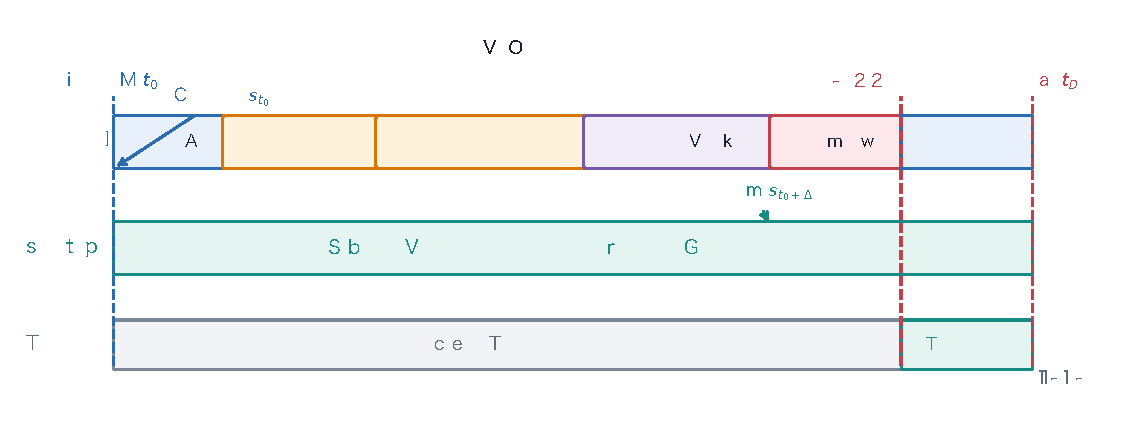
\includegraphics[width=\textwidth]{figures/v3/fig02_continuous_clock_timeline.pdf}
\caption{连续物理时钟下的一次在线决策窗口。影子元搜索与机器/AGV 执行共享同一段
wall-clock；probe 不是冻结时间的离线计算。系统在 \(t_0\) 捕获事件状态，但必须在
提交前基于 \(s_{t_0+\Delta}\) 重校验，并为停止、导出、审计和原子激活预留
commit reserve。搜索失败或重校验失败时，当前认证计划保持有效。}
\label{fig:continuous-clock}
\end{figure*}

\subsection{原子激活与安全 fallback}

Plan Revision Ledger 保存输入、输出、solver、触发事件、父版本和激活审计。新计划
只替换允许撤销的 queued/pending 运输和未开始工序；失败时回滚所有中间修改。
若不存在可安全激活候选，则执行 \(o^{\mathrm{keep}}\)，继续当前安全计划。

\begin{algorithm}[t]
\caption{\method{} 单次连续时钟在线决策}
\label{alg:online}
\begin{algorithmic}[1]
\REQUIRE 事件状态 \(s_t\)，端到端预算 \(B\)，Solver Catalog
\STATE 固定不可撤销物理前缀，生成动态候选 \(\mathcal{O}_t\)
\STATE 将 \(o^{\mathrm{keep}}\) 加入动作集合
\STATE 启动物理推进线程，继续执行当前安全计划
\WHILE{搜索预算与 probe 次数未耗尽}
    \STATE 使用 Root UCT 或逐轮淘汰选择候选和下一档预算
    \STATE 执行短 probe，记录灰盒进度并认证 incumbent
    \STATE 将无解、超时和基础设施失败按预注册成本备份
\ENDWHILE
\STATE 停止影子求解与物理推进线程，读取最新状态 \(s_{t'}\)
\STATE 对所有可行 bundle 执行 freshness、rebase 和独立审计
\STATE 删除 stale 或不可安全激活候选
\STATE 在剩余候选与 \(o^{\mathrm{keep}}\) 间按执行价值排序
\STATE 在 commit reserve 内原子激活首个通过 preflight 的计划
\STATE 若全部失败，保留当前计划；等待请求、会话和进程清零
\RETURN 决策、Plan Revision、deadline/freshness/cleanup 审计
\end{algorithmic}
\end{algorithm}

\section{系统实现}
\label{sec:implementation}

\subsection{统一求解器契约}

当前实现包括 Solver Manifest、Solver Catalog、SolverOption、真实 HTTP
ProbeEvaluator、portable incumbent、绝对 deadline、协作停止和 cleanup audit。
FJSP 首批候选为 CP-SAT、差分进化（DE）和粒子群优化（PSO）。每个 manifest 绑定
不可变镜像摘要、默认配置、预算范围、随机种子绑定和准入级别。

\subsection{物理环境与提交层}

SkyEngine 在同一 episode 中推进工序、机器、运输任务与 AGV 路径。故障触发后，
online controller 在残余 FJSP 上运行影子 probe；PlanRevisionActivator 负责计划
预检、撤销范围、缓存清理和回滚。提交层会收集本轮每个 option 的最佳认证 bundle，
在最新状态上逐个执行 freshness/rebase；sampler 首选失效时可切换到新鲜备份。
测试覆盖 future release、工序优先关系、scope 改变、commit reserve、orphan request
和物理线程失败。

\subsection{当前实现边界}

\begin{itemize}
    \item 已完成：单次机器故障、开放 FJSP 候选、连续物理推进、提交重验证和
    keep-current 基线，以及所有认证 bundle 的 commit-time freshness/rebase；
    \item 部分完成：Root MCTS、逐轮淘汰、shadow 执行价值和 stale 首选后的备份切换；
    \item 未完成：开放 MAPF meta selection、FJSP--MAPF factorized top-\(K\) 在线
    主实验、多事件 continue/switch 和 active Q。
\end{itemize}

\section{实验设计}
\label{sec:experiments}

\subsection{证据分层}

\begin{table}[t]
\centering
\caption{论文证据层级。}
\label{tab:evidence}
\begin{tabular}{P{25mm}P{42mm}P{63mm}}
\toprule
层级 & 用途 & 允许的结论 \\
\midrule
受控快照诊断 &
预算校准、纯分配器比较、事后 oracle &
不能证明在线连续时钟效果 \\
连续时钟开发实验 &
筛选动作、特征、预算和失败模式 &
只能指导方法开发，不授权主质量结论 \\
冻结独立确认 &
预注册主指标、安全 Gate 和统计检验 &
仅在协议限定范围内形成论文结论 \\
\bottomrule
\end{tabular}
\end{table}

\subsection{研究问题}

\begin{description}[leftmargin=13mm,style=nextline]
    \item[RQ1] 开放在线元调度是否优于全局最佳固定 solver/profile？
    \item[RQ2] 短 probe 是否包含预测最终执行价值的有效信息？
    \item[RQ3] 浅层 Root MCTS 是否优于逐轮淘汰？
    \item[RQ4] solver 与 probe budget 联合选择是否改善在线终局？
    \item[RQ5] keep-current 与 freshness 过滤能否降低无效重调度和 stale 提交？
    \item[RQ6] 新 solver 能否在不修改控制器固定维度的情况下接入并通过清理审计？
    \item[RQ7] deadline、物理安全、原子激活和资源清理是否始终成立？
\end{description}

\subsection{场景与数据划分}

当前冻结确认场景为 J10P5M6、两个 maze 拓扑、高严重度机器故障和 4 台 AGV。
开放方法的主实验将扩展 FJSP family、地图拓扑、故障机器和事件强度。

数据角色必须隔离：
\begin{itemize}
    \item development：特征、预算与算法筛选；
    \item calibration：预算可行性与 deadline guard；
    \item confirmation：一次性主结论；
    \item robustness：跨规模、拓扑和事件外推。
\end{itemize}
同一物理状态的不同方法共享初始状态和外生事件流；决策后允许状态自然分叉。

\subsection{对照方法}

\begin{enumerate}
    \item keep-current；
    \item 固定 CP-SAT、DE、PSO；
    \item 冻结六 profile \(T=1\) Root Search 历史基线；
    \item makespan-only 选择；
    \item 逐轮淘汰；
    \item 浅层 Root MCTS；
    \item freshness + shadow/active \(Q\)；
    \item freshness + \(Q\) + Root MCTS。
\end{enumerate}

\subsection{评价指标}

主指标为完整 episode terminal timeline 或 capped terminal makespan。辅助指标包括：
\begin{itemize}
    \item 相对全局最佳固定方法的 paired improvement；
    \item 相对同状态 oracle 的 selection regret；
    \item 完成率、P90/P95、fallback 率和 deadline overrun；
    \item 事件到提交墙钟、求解器服务时间、commit reserve；
    \item stale bundle、rebase 失败、无效激活和计划 nervousness；
    \item active request、MAPF session、进程和运输任务残留。
\end{itemize}

\subsection{统计与 Gate}

完整 episode 是在线主实验的统计单位。对同一状态的 paired difference 使用按实例和
拓扑分层 bootstrap，预注册 95\% 置信区间与失败成本。任何以下情况阻断质量主张：
\begin{equation}
\begin{split}
    &deadline\ overrun > 0,\quad invalid\ activation > 0,\\
    &physical\ violation > 0,\quad orphan\ resource > 0.
\end{split}
\end{equation}
执行价值模型还必须在按状态留组的验证中稳定优于 makespan-only 和最佳固定方法，
并通过不确定性与 abstention Gate，才允许 active。

\section{结果}
\label{sec:results}

\subsection{固定六 profile 的独立确认}

\confirmed 冻结 v2.1 在 40 个独立 cluster 上得到表~\ref{tab:v21} 的结果。该实验
证明固定候选下存在可利用的状态选择价值，并验证了 deadline-safe Root Search 的
基础设施语义。它不证明开放候选、动态多轮 switching 或 active Q。

\begin{table}[t]
\centering
\caption{六 profile \(T=1\) Root Search 独立确认结果。}
\label{tab:v21}
\begin{tabular}{lr}
\toprule
指标 & 结果 \\
\midrule
Root mean held-out cost & 459.825 \\
Global best fixed mean cost & 483.400 \\
平均绝对改善 & 23.575 \\
相对降低 & 4.88\% \\
95\% 分层 bootstrap CI & [8.625, 46.325] \\
完整 Root / 安全 fallback & 37 / 3 \\
component stress & 600 / 600 PASS \\
normal / forced-deadline stress & 25/25，25/25 PASS \\
最终 active request / MAPF session & 0 / 0 \\
\bottomrule
\end{tabular}
\end{table}

\begin{figure*}[t]
\centering
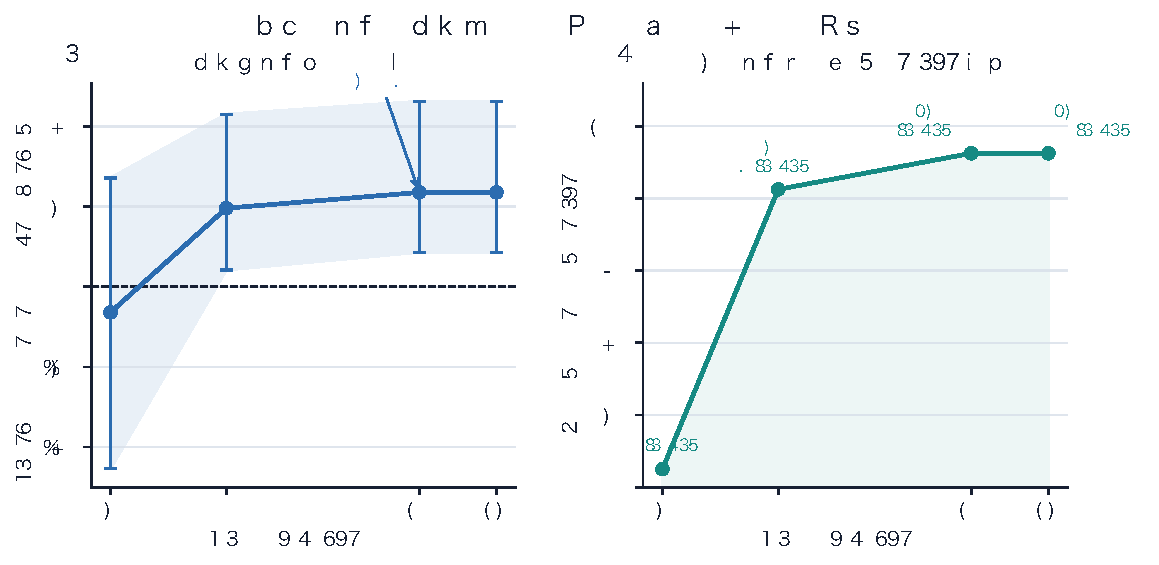
\includegraphics[width=\textwidth]{figures/v3/fig03_budget_quality_confirmation.pdf}
\caption{\confirmed 冻结六 profile 独立确认中的预算--质量--覆盖率关系。左图为相对
全局最佳固定 profile 的 40 状态配对改善及 95\% 分层 bootstrap 置信区间；右图为
Root 在相应预算内完成选择而不使用 fallback 的覆盖率。2\,s 预算只有 5.0\% coverage，
5\,s 后收益转正，10\,s 与 12\,s 的均值和 coverage 相同。}
\label{fig:budget-quality-confirmation}
\end{figure*}

图~\ref{fig:budget-quality-confirmation} 表明，极短 deadline 下的主要瓶颈不是排序精度，
而是候选能否在预算内完成。2\,s 的平均改善为 \(-6.400\)，置信区间跨越 0；5\,s
coverage 提升至 82.5\%，平均改善为 19.625；10\,s 时 coverage 为 92.5\%，平均改善
达到 23.575，继续增加到 12\,s 未带来额外收益。该曲线支持把 solver 质量和
deadline coverage 联合报告，而不能只给单一最终 makespan。

\begin{figure*}[t]
\centering
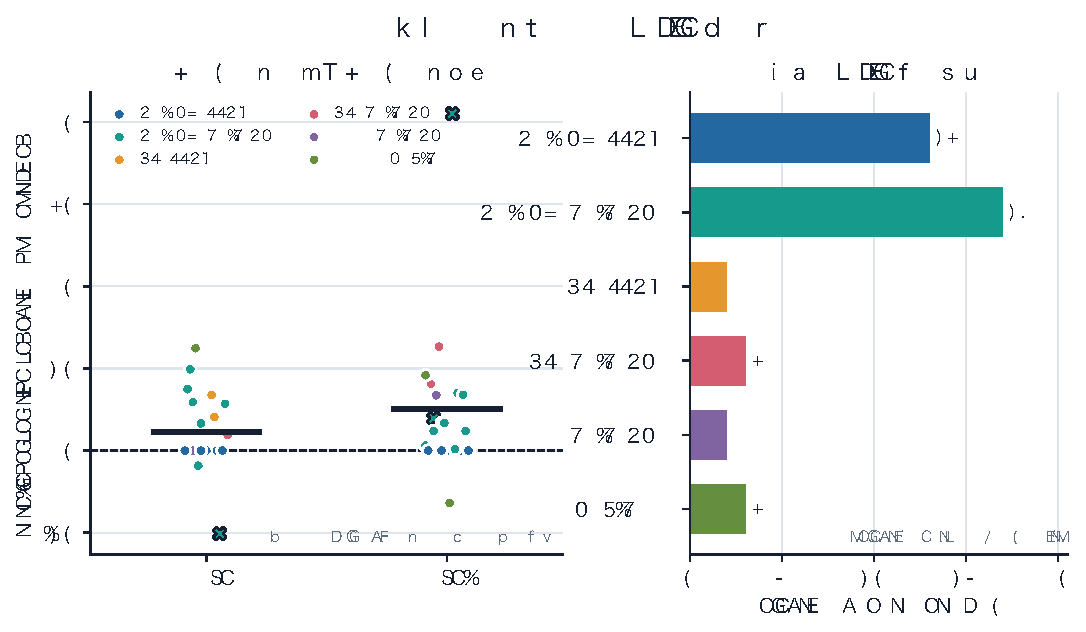
\includegraphics[width=\textwidth]{figures/v3/fig04_state_profile_confirmation.pdf}
\caption{\confirmed 冻结六 profile 独立确认中的状态依赖互补性。左图按拓扑展示每个
状态相对全局最佳固定 profile 的归一化改善；黑边 X 表示使用安全 fallback 的状态，
短横线表示拓扑内均值。右图为 Root 的 profile 选择次数。归一化仅用于跨状态可视化，
正式主指标仍为表~\ref{tab:v21} 的绝对配对改善。}
\label{fig:state-profile-confirmation}
\end{figure*}

图~\ref{fig:state-profile-confirmation} 中 23/40 状态改善、14/40 持平、3/40 退化；
选择覆盖全部六个 profile，各 profile 至少被选择两次，选择熵为 2.04 bits。
held-out oracle 相对全局最佳固定方法的平均 headroom 为 30.700，Root 关闭了
76.79\% 的 oracle regret。这说明固定候选内存在状态选择价值，但结论只适用于冻结
实例、拓扑、机器故障、六 profile 和 deadline policy。

\subsection{连续时钟在线闭环验收}

\development 在真实 CP-SAT、DE、PSO 服务上，toy episode 与 J10P5M6 开发实验均
完成连续物理推进、bundle 认证、commit-time rebase 和原子激活。最近的多状态
cohort 共包含：
\begin{equation}
    30\ \text{全预算}
    + 15\ \text{短预算}
    + 5\ \text{keep-current}
    = 50\ \text{episodes}.
\end{equation}
5 个状态的 snapshot、problem 和 scope hash 在不同动作间严格配对；全部 episode
结束后 solver health 通过。全预算 30/30 probe 可行、26/30 激活；短预算 14/15
probe 可行、14/15 激活。全预算未激活的 4 次均来自同一状态的 DE/PSO stale bundle，
系统正确保留当前计划。

\subsection{求解器互补性}

\begin{figure*}[t]
\centering
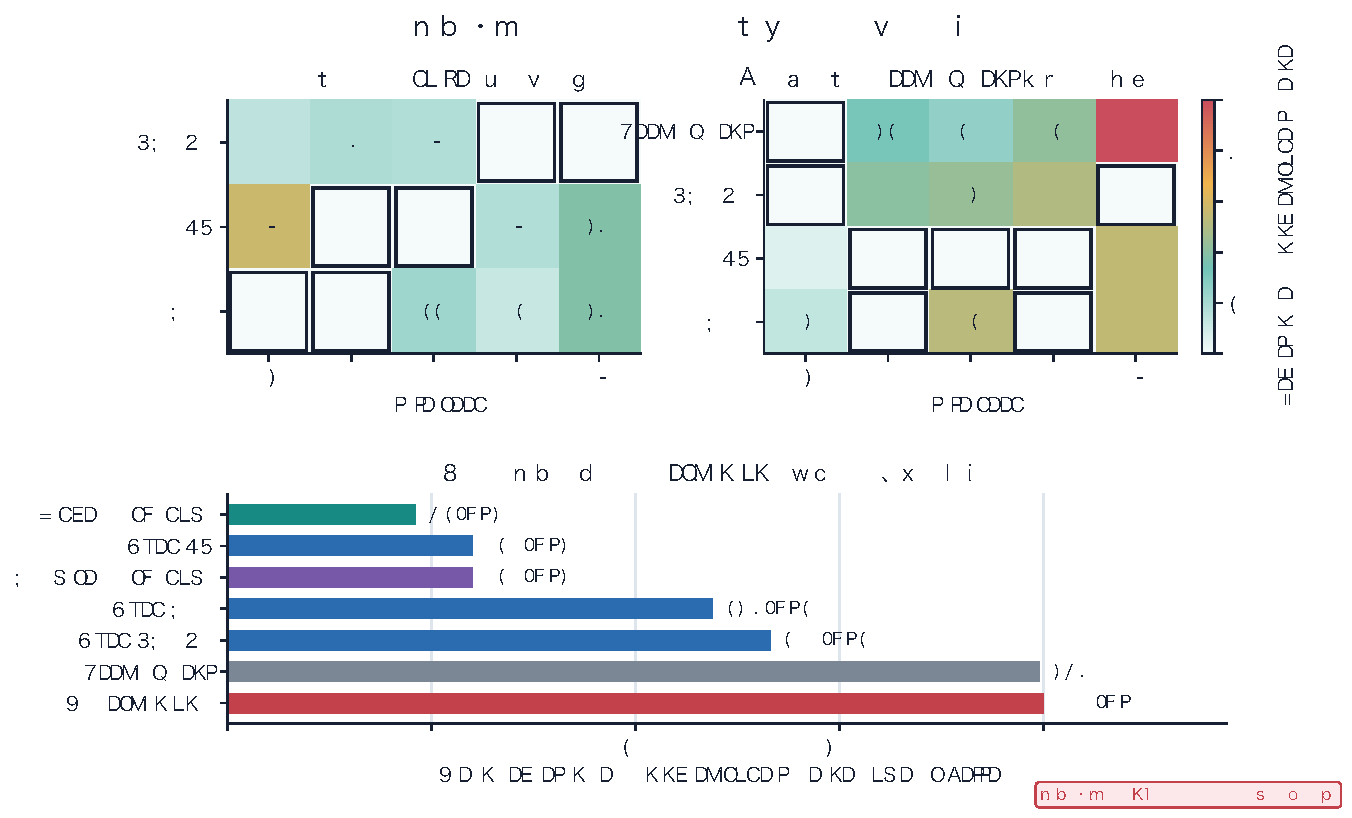
\includegraphics[width=\textwidth]{figures/v3/fig05_execution_value_development.pdf}
\caption{\development 五个严格配对状态上的动作价值开发诊断，不构成正式质量结论。
(a) 全预算下各 solver 相对同状态 oracle 的剩余 episode timeline regret；
(b) 短预算加入 keep-current 后的 regret；黑框表示进入状态最优集合；
(c) 严格 leave-one-state-out 下，不同固定策略、makespan-only 和 shadow \(Q\) 的
平均 regret。\(Q\) 仅用于离线诊断，当前未授权 active。}
\label{fig:execution-value-development}
\end{figure*}

\development 图~\ref{fig:execution-value-development}(a) 中，PSO 在 seed53 最优，
DE/PSO 在 seed54 并列最优，DE 在 seed55 最优，CP-SAT 在 seed56 和 seed57 最优。
三个 solver 都至少在一个状态进入最优集合，说明候选具有互补性。全预算的两次重复
终局 target 最大极差为 0，但该稳定性不能推广到其他预算。

\subsection{预算与 keep-current}

图~\ref{fig:execution-value-development}(b) 中，短预算 oracle 相对始终
keep-current 平均减少 39.8 个物理步，但 seed53 中 keep-current 与 CP-SAT
fallback 终局相同；由于前者不产生额外 probe 开销，oracle 选择 keep-current。
这说明重调度本身不是无条件有益。对 15 个 state-solver 配对，全预算改为短预算后
10 个更好、3 个相同、2 个更差。seed57 中 DE/PSO 全预算约运行 3.3 秒，物理状态
推进 3 步并导致 repair scope 改变；短预算避免 stale，但仍不如 CP-SAT。因此
\(solver\) 与 \(budget\) 必须共同构成动作。

\subsection{makespan-only 与状态执行价值}

\development 图~\ref{fig:execution-value-development}(c) 使用严格
leave-one-state-out。裸 makespan 在 5 个状态中全部选错，平均 regret 为 40.0；
最佳固定 DE 为 12.0。透明 ridge 的平均 regret 降至 9.2，但在 seed54 仍产生
40 步 regret，且样本只有 5 个独立状态。因此：
\begin{equation}
    \texttt{execution\_value\_active\_authorized} = \texttt{false}.
\end{equation}
当前结果只支持扩大 shadow 数据采集，不能声称价值模型已经优于强基线。

\subsection{统一动作 schema 的 30 状态开发结果}

\begin{figure*}[t]
\centering
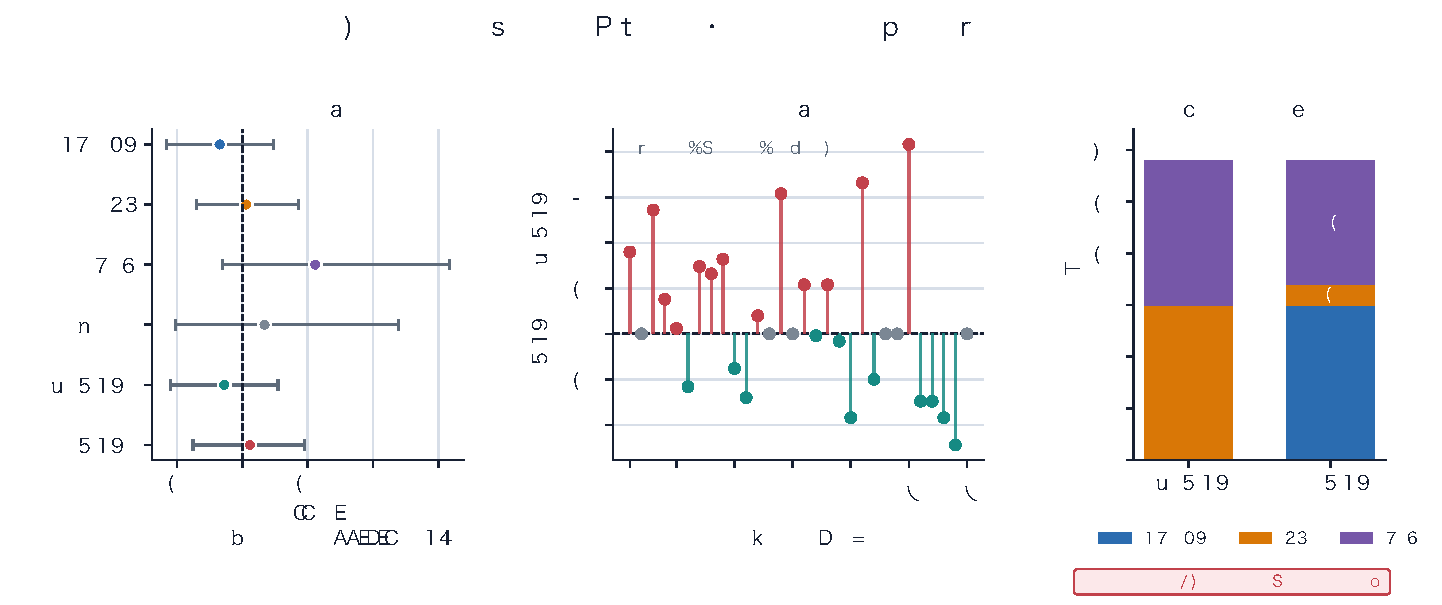
\includegraphics[width=\textwidth]{figures/v3/fig06_online_meta_30state_development.pdf}
\caption{\development 统一 keep-current/solver/config/budget 动作 schema 后的
30 状态、7 策略配对在线开发实验。(a) 各策略相对 keep-current 的终局 timeline
配对差值，负值更好；(b) 为 CP-SAT 配置 1000\,ms 最小可辨识预算后，校准 MCTS
相对原始 MCTS 的逐状态变化；(c) 两种 MCTS 的最终 solver 选择次数。校准恢复了
CP-SAT 覆盖，但未改善平均终局，不能作为正式质量结论。}
\label{fig:online-meta-30state-development}
\end{figure*}

\development 图~\ref{fig:online-meta-30state-development} 汇总 seeds 1000--1029。
每个 action-independent 状态均完成 snapshot、problem、scope hash 配对，并通过
decision--outcome 最终动作一致性审计。30 个状态乘 7 种策略共得到 210 个 episode；
deadline、commit reserve、solver health、物理时钟和运输唯一性失败均为 0。原始
MCTS 的平均终局为 498.2，相对 keep-current 的配对差值为 \(-5.5\)，95\% bootstrap
置信区间为 \([-21.90,10.93]\)；固定 CP-SAT 为 496.8，逐轮淘汰为 510.53。
因此当前数据不支持 MCTS 稳定优于强固定方法。

原始 MCTS 在 500\,ms 首轮从未从 CP-SAT 得到可行 incumbent，最终选择为 DE 15 次、
PSO 14 次和 keep-current 1 次。校准版从 option metadata 读取最小可辨识预算：
CP-SAT 首轮 1000\,ms，DE/PSO 首轮 500\,ms。CP-SAT 首轮可行覆盖恢复到 28/30，
最终被选择 15 次；但校准版平均终局为 506.0，相对原始 MCTS 平均退化 7.8，
95\% 区间为 \([-6.10,22.53]\)，11/30 状态改善、6/30 持平、13/30
退化。该消融表明：
\begin{equation}
    \text{candidate coverage}
    \not\Rightarrow
    \text{online execution value}.
\end{equation}
探测分配必须同时考虑首次可行概率、运行时引起的状态漂移，以及最新状态上候选对
完整在线过程的执行价值；仅通过固定的 solver-specific 预算门槛无法完成三者权衡。
active \(Q\) 仍保持禁用。

\subsection{开放元调度主结果占位}

\pending 表~\ref{tab:mainplaceholder} 必须由冻结独立确认协议一次性填充。开发数值
不得复制到该表。

\begin{table}[t]
\centering
\caption{开放在线元调度主结果（独立确认占位）。}
\label{tab:mainplaceholder}
\small
\begin{tabular}{P{38mm}cccc}
\toprule
方法 & Mean & P95 & 回退率 & Regret \\
\midrule
Keep-current & \pending & \pending & -- & \pending \\
Global best fixed & \pending & \pending & \pending & \pending \\
Successive halving & \pending & \pending & \pending & \pending \\
Root MCTS & \pending & \pending & \pending & \pending \\
Freshness + \(Q\) & \pending & \pending & \pending & \pending \\
Freshness + \(Q\) + MCTS & \pending & \pending & \pending & \pending \\
\bottomrule
\end{tabular}
\end{table}

\section{讨论}
\label{sec:discussion}

\subsection{当前证据说明了什么}

第一，固定候选的独立确认已经证明动态 FJSP--MAPF 状态中存在 solver portfolio
headroom，且 deadline-safe Root Search 可以在限定范围内实现正收益。第二，连续
时钟开发实验表明，离线 FJSP makespan 无法可靠代表在线执行质量；solver runtime、
运输结构和提交时状态漂移都可能改变最终排序。第三，keep-current、solver 和 budget
必须形成统一动作，而不是在事件发生后强制重调度。

\subsection{为什么不展开未来制造状态树}

深层制造状态 MCTS 需要反复模拟 FJSP、AGV、MAPF、故障和物理时间，计算成本高且
模型误差会随深度累积。项目已有 open-loop UCT 未优于 Root Search 的冻结负结果。
因此本文让 MCTS 只承担 ``计算预算分配''，把长期执行价值交给可校准的 \(Q\) 估计，
把物理可行性留给确定性审计。

\subsection{为什么 freshness 不能交给学习模型}

价值模型可能估计 stale 风险，但 scope、不可撤销运输和证书一致性属于硬约束。
学习误差不能授权违反硬约束的计划。正确顺序是先在最新状态上确定性删除不可提交
候选，再在安全候选之间进行风险排序。

\subsection{开放性与可复现性的关系}

运行时 catalog 可以开放，但正式实验必须冻结。开放性指新 solver 能通过稳定契约
加入候选，不代表 confirmation 时允许候选集合任意变化。每次正式实验仍需冻结
manifest、镜像摘要、配置 schema、预算、seed 和统计协议。

\section{局限性与后续工作}
\label{sec:limitations}

\begin{enumerate}
    \item 当前开放在线链路只动态选择 FJSP solver；MAPF 仍由现有路由器处理。
    \item 当前主场景为单次机器故障，尚未覆盖多事件 episode、随机到达和路径阻塞。
    \item 执行价值模型只在 5 个独立状态上完成留状态开发评估；30 状态新 cohort
    尚未用于预注册的模型训练和留组验证，因此不能 active。
    \item 当前 45 维特征是透明表格特征；数据充分后才考虑异构图价值网络。
    \item 尚未完成跨 FJSP family、地图类型、AGV 数量和事件类型的外部有效性验证。
    \item 30 状态开发 cohort 使用三条容器 lane 并行运行，宿主机 CPU 仍共享；
    正式确认必须进行资源隔离或单 lane 顺序复跑，并报告 wall-clock 重复性。
    \item 离散时间和仿真环境不能替代真实工厂中的运动学、通信和安全认证。
\end{enumerate}

下一阶段优先级为：在已统一的 keep-current/solver/config/budget 动作 schema 上，
用 30 状态 cohort 校准 ``首次可行概率 + 探测运行时 + 最新状态执行价值'' 的联合
分配；采用严格按状态留组的验证，比较原始 MCTS、校准 MCTS、最佳固定方法和
makespan-only。只有验证稳定通过后，才冻结 active Q 与开放元调度 confirmation
协议。

\section{结论}
\label{sec:conclusion}

本文提出 \method{}，研究连续物理时钟下动态 FJSP--MAPF 的开放式、截止期安全
solver-portfolio 元调度。框架使用可扩展 Solver Catalog 表达 solver、配置与预算，
以短 probe 和浅层 Root MCTS 分配计算资源，并通过最新状态 freshness/rebase、
独立审计和原子激活保证提交安全。状态执行价值进一步把选择目标从 solver 内部
makespan 扩展到完整 episode 成本，并把保持当前计划纳入动作空间。

冻结六 profile 基线已在限定范围内完成独立确认；连续时钟开发实验进一步显示
solver 互补性、预算效应以及 makespan-only 的系统性不足。开放候选、active 执行价值
和 MCTS 相对逐轮淘汰的最终收益仍需独立确认。本文因此把当前结论限定为：
方法主链路已具备可执行和可审计基础，状态执行价值具有明确研究前景，但最终算法优势
尚不能由开发结果替代。

\section*{可复现性说明}

当前主要证据：
\begin{itemize}
    \item 固定六 profile 独立确认：
    \par
    \path{artifacts/skycausal_publication_confirmation_v2_1_09760697/}；
    \item 状态执行价值开发分析：
    \par
    \path{artifacts/skycausal_execution_value_analysis_dev_v0/analysis.json}；
    \item 统一动作 schema 的 30 状态在线开发分析：
    \par
    \path{artifacts/skycausal_online_meta_unified_action_dev_v1/analysis_30state_calibrated.json}；
    \item 论文图表生成器与证据 manifest：
    \par
    论文目录中的 \path{scripts/generate_v3_figures.py}，
    \path{figures/v3/figure_manifest.json}；
    \item 开放 Solver Catalog、probe 和在线控制器：
    \par
    \path{codebase/SkyEngine/experiment/skycausal/}；
    \item 当前 SkyCausal 回归测试：379 项通过。
\end{itemize}
图表可由 SkyEngine 虚拟环境中的 Python 运行
\path{scripts/generate_v3_figures.py} 重建。manifest 记录正式与开发数据源的
SHA256、每张图的证据等级及 PDF/PNG 哈希。

\bibliographystyle{plainnat}
\bibliography{references_skycausal_v3}

\end{document}
